\documentclass[11pt,a4paper]{article}
\usepackage{listings}
\usepackage[utf8]{inputenc}
\usepackage{mathtools}
\usepackage[norsk]{babel}
\usepackage{graphicx}
\usepackage{gensymb}
\usepackage{wasysym}
\usepackage{hyperref}
\usepackage{setspace}
\usepackage{tikz}
\usepackage{amsthm}
\usepackage{amsmath}
\usepackage{mathrsfs}
\usepackage{amssymb}
\usepackage{color}
\usepackage{rotating}
\usepackage{pgfplots}
\usepackage{algorithmicx}
\usepackage{fancyvrb}



\usetikzlibrary{arrows}
\usetikzlibrary{shapes, automata}


\newcommand{\intt}{integritetsregler}
\newcommand{\inttt}{integritetsregel}
\newcommand{\Intt}{Integritetsregler}
 
\definecolor{dkgreen}{rgb}{0,0.6,0}
\definecolor{gray}{rgb}{0.5,0.5,0.5}
\definecolor{mauve}{rgb}{0.58,0,0.82}


\lstset{ %
  language=Java,                % the language of the code
  basicstyle=\small\rmfamily,           % the size of the fonts that are used for the code
  numbers=none,                   % where to put the line-numbers
  numberstyle=\small\color{gray},  % the style that is used for the line-numbers
  stepnumber=1,                   % the step between two line-numbers. If it's 1, each line 
                                  % will be numbered
  numbersep=5pt,                  % how far the line-numbers are from the code
  backgroundcolor=\color{white},      % choose the background color. You must add \usepackage{color}
  showspaces=false,               % show spaces adding particular underscores
  showstringspaces=false,         % underline spaces within strings
  showtabs=false,                 % show tabs within strings adding particular underscores
  frame=,                   % adds a frame around the code
  rulecolor=\color{gray},        % if not set, the frame-color may be changed on line-breaks within not-black text (e.g. commens (green here))
  tabsize=2,                      % sets default tabsize to 2 spaces
  captionpos=b,                   % sets the caption-position to bottom
  breaklines=true,                % sets automatic line breaking
  breakatwhitespace=false,        % sets if automatic breaks should only happen at whitespace
  title=\lstname,                   % show the filename of files included with \lstinputlisting;
                                  % also try caption instead of title
  keywordstyle=\bfseries\color{black},          % keyword style
  commentstyle=\color{dkgreen},       % comment style
  stringstyle=\color{mauve},         % string literal style
  escapeinside={\%*}{*)},            % if you want to add LaTeX within your code
  morekeywords={*,..,}               % if you want to add more keywords to the set
}

\setlength{\parskip}{5mm}

\newtheoremstyle{def}
	{3pt}	% Space above
	{3pt}	% Space below
	{\itshape}		% Font
	{}		% Indent
	{\bfseries}		% Head font
	{:}		% Head punct.
	{.5em}	% Space after head
	{}		% Head spec

\theoremstyle{def}
\newtheorem{definition}[subsection]{Definisjon}

%\newenvironment{definition}[1][Definisjon]{\begin{trivlist}
%\item[\hskip \labelsep {\bfseries #1}]}{\end{trivlist}}

\title{Notater: INF2220}
\author{Veronika Heimsbakk \\ 
veronahe@student.matnat.uio.no}
\begin{document}

\maketitle{}
\tableofcontents
\newpage{}

\section*{Introduksjon}
Dette er notater til kurset INF2220--Algoritmer og datastrukturer ved Universitetet i Oslo. Disse notatene er i all hovedsak basert på forelesningsfoiler, egne notater og læreboka. Brukes til repetisjon før eksamen og som notater under eksamen. Merk at notatene helt sikkert inneholder feil og mangler.


%%% KJØRETID %%%
\section{Kjøretid}

\begin{definition}
\emph{\textbf{O-notasjon}}
La $f$ og $g$ være funksjoner $f,g: \mathcal{N} \rightarrow \mathcal{R}^+$. Sier at $\textbf{f(n) = O(g(n))}$ hvis det eksisterer positive heltall $c$ og $n_0$ slik at for hvert heltall $n \geq n_0$,
$$f(n) \leq c g(n).$$
Når $f(n) = O(g(n))$, sier vi at $g(n)$ er \textbf{upper bound} for $f(n)$, eller mer presist at $g(n)$ er \textbf{asymptotic upper bound} for $f(n)$.
\end{definition}

\begin{table}[h!]
\centering
\begin{tabular}{rl}
\textbf{Funksjon}&\textbf{Navn}\\
$1$&Konstant\\
$\log n$&Logaritmisk\\
$n$&Lineær\\
$n \log n$&\\
$n^2$&Kvadratisk\\
$n^3$&Kubisk\\
$2^n$&Eksponensiell\\
$n!$&\\
\end{tabular}
\label{tab:ofunc}
\caption{Vanlige funksjoner for O$(n)$}
\end{table}

\begin{figure}[h!]
\centering
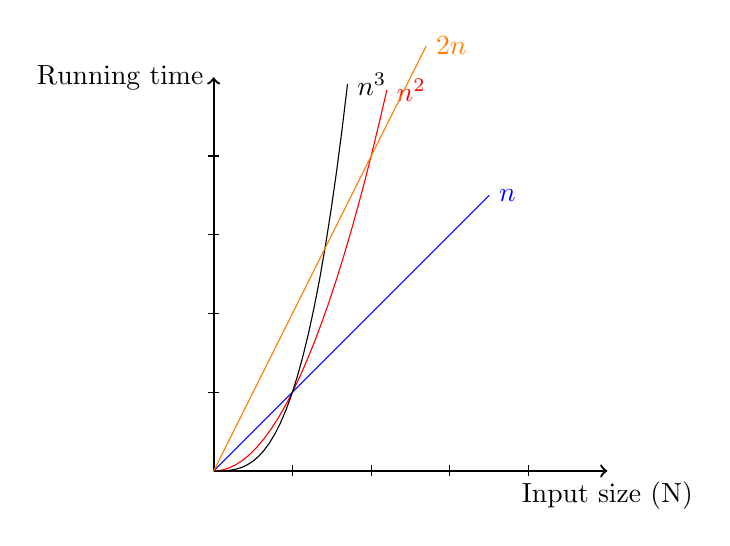
\begin{tikzpicture}
\draw[thick, ->] (0,0) -- (5,0) node[below] {Input size  (N)};
\draw[thick, ->] (0,0) -- (0,5) node[left] {Running time};

\foreach \x in {1,2,3,4}
	\draw (\x cm, 2pt) -- (\x cm, -2pt);
\foreach \y in {1,2,3,4}
	\draw (2pt, \y cm) -- (-2pt, \y cm);

\draw[red, domain=0:2.2] plot (\x, {\x^2}) node[right]{$n^2$};
\draw[blue, domain=0:3.5] plot (\x, {\x}) node[right] {$n$};
\draw[black, domain=0:1.7] plot (\x, {\x^3}) node[right] {$n^3$};
\draw[orange, domain=0:2.7] plot (\x, {2*\x}) node [right] {$2n$};
\end{tikzpicture}
\label{fig:ofunc}
\caption{Noen funksjoner for O$(n)$.}
\end{figure}

\subsection{Analyse av kjøretid}
Når man analyserer en algoritme, så må man se på \textit{stegene} den bruker og analysere de hver for seg. Ta for eksempel denne kodesnutten:
\begin{Verbatim}[frame=single]
for (i = 0; i < n; i++)
  for (j = 0; j < m; j++)
    array[i][j] = 0;
\end{Verbatim}
Her har vi to steg: løkken som går $n$ steg, og løkken som går $m$ steg. Den første løkken går i O(N), mens den andre løkken går i O(M). Siden den innerte løkken går M ganger N ganger (siden den er nestet i den ytterste løkken). Så vil den totale tiden være O(M) $\times$ O(N), dermed O$(n^2)$.


%%% TRÆR %%%
\section{Trær}

\begin{definition}
\emph{\textbf{Tre}}
Et \textbf{tre} er en samling \textbf{noder}. Et ikke-tomt tre består av en \textbf{rot}-node, og null eller flere ikke-tomme \textbf{subtrær}. Fra roten går en \textbf{rettet kant} til roten i hvert subtre.
\end{definition}

% Traversering
\subsection{Traversering}
\begin{description}
\item[Pre-order] rot, venstre barn, høyre barn
\item[In-order] venstre barn, rot, høyre barn
\item[Post-order] venstre barn, høyre barn, rot
\end{description}

\begin{lstlisting}
/* IN-ORDER TRAVERSAL */

public void inOrder (Node node) {
	if (node != null) {
		inOrder(node.left);
		// do something with the node
		inOrder(node.right);
	}
}

/* PRE-ORDER TRAVERSAL */

public void preOrder (Node node) {
	if (node != null) {
		// do something with the node
		preOrder(node.left);
		preOrder(node.right);
	}
}

/* POST-ORDER TRAVERSAL */

public void postOrder (Node node) {
	if (node != null) {
		postOrder(node.left);
		postOrder(node.right);
		// do something with the node
	}
}
\end{lstlisting}

% Terminologi
\subsection{Terminologi}
\begin{definition}
\emph{\textbf{Sti}}
En sti fra node $n_1$ til $n_k$ er definert som en sekvens $n_1, n_2, \dots, n_k$, slik at $n_i$ er forelder til $n_{i+1}$ for $1 \leq i \leq k$.
\end{definition}
\begin{definition}
\emph{\textbf{Lengde}}
Antall \textit{kanter} på veien; $k-1$.
\end{definition}
\begin{definition}
\emph{\textbf{Dybde}}
Definert av den unike veien fra roten til noden. Rotens dybde er 0.
\end{definition}
\begin{definition}
\emph{\textbf{Høyde}}
Definert som lengden av den \textit{lengste} veien fra noden til en løvnode. Alle løvnoder har høyde 0. Høyden til et tre er lik høyden til roten.
\end{definition}


\newpage
%%% BINÆRTRÆR %%%
\subsection{Binært søketre}

\begin{definition}
\emph{\textbf{Binært søketre}}
Et binært søketre (BST) er et \textbf{ordnet} binært tre. Følgende kriterier må være oppfylt for at treet skal være et BST:
\begin{itemize}
\item
Verdiene i \textbf{venstre} subtre er \textbf{mindre} enn noden i seg selv.
\item
Verdiene i \textbf{høyre} subtre er \textbf{større} enn noden i seg selv.
\item
Venstre og høyre subtre må også være binære søketrær.
\item
Hver node kan ha maksimum to barn.
\item
Det eksisterer en \textbf{unik} sti fra roten til enhver node i treet.
\end{itemize}
\end{definition}

\begin{figure}[h!]
\centering
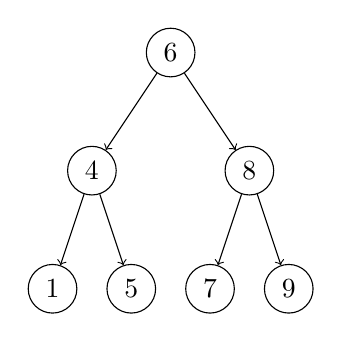
\begin{tikzpicture}[->,every node/.style={circle, draw=black}, 
				   level 1/.style={sibling distance=20mm},
				   level 2/.style={sibling distance=10mm}]
\node{6}
	child {node {4}
		child {node {1}}
		child {node {5}}
	}
	child {node {8}
		child {node {7}}
		child {node {9}}
	}
;
\end{tikzpicture}
\label{fig:simplebst}
\caption{Eksempel på et binært søketre.}
\end{figure}

\subsubsection{Tidkompleksitet}
\begin{table}[h!]
\centering
\begin{tabular}{rll}
&Average&Worst case\\
\textbf{Plass} & O($n$) & O($n$)\\
\textbf{Søk} & O($\log n$) & O($n$)\\
\textbf{Innsetting} & O($\log n$) & O($n$)\\
\textbf{Sletting} & O($\log n$) & O($n$)\\
\end{tabular}
\label{tab:obst}
\caption{Tidkompleksitet for BST.}
\end{table}

\newpage
\subsubsection{Søking}
\begin{Verbatim}[frame=single]
function find(key, node):
  if node = Null or node.key = key then
    return node
  else if key < node.key then
    return find(key, node.left)
  else
    return find(key, node.right)
\end{Verbatim}

\subsubsection{Sette inn}
\begin{Verbatim}[frame=single]
function insert(root, data):
  if (!root)
    root = new Node(data)
  else if (data < root.data)
    insert(root.left, data)
  else if (data > root.data)
    insert(root.right, data)
\end{Verbatim}

\subsection{Rød-svarte trær}
\begin{definition}
\emph{\textbf{Rød-svart tre}}
En datastruktur som er et \textbf{selv-balanserende} binært søketre. Følgende skal gjelde for et rød-svart tre:
\begin{enumerate}
\item
En node er enten rød eller sort.
\item
Roten er sort.
\item
Alle løvnoder (NIL) er sorte---alle løvnoder har samme farge som roten.
\item
Enhver røde node må ha to sorte barn.
\item
Enhver sti fra roten til en løvnode skal inneholde samme antall sorte noder.
\end{enumerate}
Dette sikrer at høyden på et slikt tre er maks $2\times\log_2(N+1)$.
\end{definition}


\tikzset{
	treenode/.style = {align=center, inner sep=0pt},
	% Sorte noder
	node_black/.style = {treenode, circle, white,
						font=\bfseries, draw=black,
						fill=black, text width=0.8cm},
	% Røde noder
	node_red/.style = {treenode, circle, red, draw=red,
						text width=0.8cm, very thick},
	% Null-pekere
	node_null/.style = {white, treenode, rectangle, draw=black, fill=black,
						minimum width=0.3cm, minimum height=0.3cm}
}


\subsubsection{Eksempel på innsetting}
\begin{figure}[h!]
\centering
\begin{tabular}{p{4cm}p{4cm}p{4cm}}
1&2&3\\
\scalebox{0.8}{
\begin{tikzpicture}[level 1/.style={sibling distance=20mm},
				   level 2/.style={sibling distance=10mm, level distance=10mm}]
\node[node_black]{41}
	child {node[node_red] {38}
		child {node[node_null] {nil}}
		child {node[node_null] {nil}}
	}
	child {node [node_null] {nil}}
;
\end{tikzpicture}
}
&
\scalebox{0.8}{
\begin{tikzpicture}[level 1/.style={sibling distance=20mm},
				   level 2/.style={sibling distance=10mm, level distance=10mm}]
\node[node_black]{38}
	child {node[node_red] {31}}
	child {node [node_red] {41}}
;
\end{tikzpicture}
}
&
\scalebox{0.8}{
\begin{tikzpicture}[level 1/.style={sibling distance=20mm},
				   level 2/.style={sibling distance=10mm}]
\node[node_black]{38}
	child {node[node_black] {31}
		child {node[node_null] {nil}}
		child {node[node_red] {12}
		}
	}
	child {node [node_black] {41}}
;
\end{tikzpicture}
}
\\
Setter inn 41 og 38 etter reglene. 
& Når 31 nå kommer inn, så må vi snu på treet og farge om 38 og 41. 
& Siden løvnodene var røde når 12 skal inn, så må 31 og 41 farges om. 41 skal farges iht. regel nr. 3.\\
\scalebox{0.8}{
\begin{tikzpicture}[level 1/.style={sibling distance=20mm},
				   level 2/.style={sibling distance=10mm}]
\draw[black] (0,1) node[above]{4.};
\node[node_black]{38}
	child {node[node_red] {19}
		child {node[node_black] {12}}
		child {node[node_black] {31}}
	}
	child {node [node_black] {41}}
;
\end{tikzpicture}
}
&
\scalebox{0.8}{
\begin{tikzpicture}[level 1/.style={sibling distance=20mm},
				   level 2/.style={sibling distance=10mm}]
\draw[black] (0,1) node[above]{5.};
\node[node_black]{38}
	child {node[node_red] {19}
		child {node[node_black] {12}
			child{node[node_red] {8}}
			child{node[node_null] {nil}}
		}
		child {node[node_red] {31}}
	}
	child {node [node_black] {41}}
;
\end{tikzpicture}
}
&\\
Når 19 nå kommer inn, så må vi igjen snu på treet for å opprettholde reglene til et BST. Farger nodene på nytt iht. reglene for rød-svarte trær.
&
Til slutt setter vi inn 8 som løvnode til 12. Her trenger vi ikke å snu eller fargelegge.
\end{tabular}
\label{fig:rseks}
\caption{Eksempel på innsetting av tallene 41, 38, 31, 12, 19 og 8 i et rød-svart tre.}
\end{figure}

\vspace{20pt}
 
\begin{figure}[h!]
\begin{lstlisting}[frame=single]
/* Red-black insertion */

public void put (Key key, Value val) {
	root = put(root, key, val);
	root.color = BLACK;
}

// insert key-value pair in subtree with root node
private Node put (Node node, Key key, Value val) {
	if (node == null) return new Node(key, val, RED, 1);

	int cmp = key.compareTo(node.key);
	if (cmp < 0) 
		node.left = put(node.left, key, val);
	if else (cmp > 0)
		node.right = put (node.right), key, val);
	else 
		node.val = val;

	if ( isRed(node.right) && !isRed(node.left) ) 
		node = rotateLeft(node);
	if ( isRed(node.left) && isRed(node.left.left) ) 
		node = rotateRight(node);
	if ( isRed(node.left) && isRed(node.right) ) 
		flipColors(node);
	node.N = size(node.left) + size(node.right) + 1;

	return node;
}
\end{lstlisting}
\caption{Eksempel på innsetting i rødsvart tre \cite{redblack}.}
\end{figure}

\begin{table}[h!]
\centering
\begin{tabular}{rll}
&Average&Worst case\\
\textbf{Plass} & O($n$) & O($n$)\\
\textbf{Søk} & O($\log n$) & O($\log n$)\\
\textbf{Innsetting} & O($\log n$) & O($\log n$)\\
\textbf{Sletting} & O($\log n$) & O($\log n$)\\
\end{tabular}
\label{tab:obst}
\caption{Tidkompleksitet for rød-svarte trær.}
\end{table}

%%% B-TRÆR %%%
\subsection{B-trær}


%%% MAPS %%%
\section{Maps}

%%% HASHING %%%
\section{Hashing}
Idéen i hashing er å lagre alle elementene i en array (hashtabell) og la verdien i elementet $x$ bestemme indeksen til $x$ i hashtabellen. Egenskaper til en god hash-funksjon er at den er rask å beregne, kan gi alle mulige verdier fra 0 til tabellens størrelse $-1$. Og den git en god fordeling utover tabellindeksene. En hashtabell tilbyr innsetting, sletting og søking med konstant tid.

\subsection{Hash-funksjoner}
\paragraph{Eksempel} med heltall som nøkkel, begrenset antall tabellindekser. La hashfunksjonen være \texttt{hash(x, taleSize) = x mod tableSize}. Husk at hvis \texttt{tableSize} er 10 og alle nøklene slutter på 0, vil alle elementene havne på samme indeks. Huskeregel for dette: la alltid tabellstørrelsen være et primtall. Funksjonen under summerer verdiene til hver bokstav. Dette er en dårlig fordeling dersom tabellstørrelsen er stor.
\begin{lstlisting}
int hash (String key, int tableSize) {
	int hashValue = 0;
	for (i = 0; i < key.length(); i++) 
		hashValue+= key.charAt(i);
	return (hashValue % tableSize);
}
\end{lstlisting}

\subsection{Forskjellige typer hash-tabeller}
\begin{itemize}
\item
\textbf{Seprate chaining} er en hash-tabell hvor hver indeks peker til en liste av elementer.
\item
\textbf{Probing} er rommet mellom hver indeks.
\begin{itemize}
\item
\textit{Lineær probing}; intervallene er satt (normalt 1).
\item
\textit{Kvadratisk probing}; intervallene øker med å legge til et kvadratisk polynom ved startverdi gitt av hashberegningen.
\item
\textit{Dobbel hashing}; intervallene er gitt av en annen hash-funksjon.
\end{itemize}
\end{itemize}

\begin{table}[h!]
\centering
\begin{tabular}{c|c|c|c}
Index & Linear probing & Quadratic probing & Separate chaining\\
\hline
0 & 9679 & 9679 &\\
1 & 4371 & 4371 & \\
2 & 1989 & &\\
3 & 1323 & 1323 & 1323 $\rightarrow$ 6173\\
4 & 6173 & 6173 & 4344\\
5 & 4344 & 4344 &\\
6 & & &\\
7 & & &\\
8 & & 1989 &\\
9 & 4199 & 4199 & 4199 $\rightarrow$ 9679 $\rightarrow$ 1989\\
\end{tabular}
\label{tab:hash}
\caption{Eksempel på hashing.}
\end{table}
I tabell \ref{tab:hash} har vi forskjellige hash-tabeller på tallene \{4371, 1323, 4199, 4344, 9679, 1989\} som skal settes inn i en tabell på størrelse 10, og med hash-funksjon \texttt{H(X) = X mod 10}.

\paragraph{Lineær probing} her tar man tallet og setter inn i hash-funksjonen. Så for første tall (4371) vil indeksen bli 1. Hvis indeksen er opptatt, så plusser man på 1.

\paragraph{Kvadratisk probing} er så og si det samme, men i stedet for å legge til 1 hvis indeksen er opptatt, så legger man på $1^2, 2^2, 3^2,\dots$

\paragraph{Dobbel probing} her lager vi en ny hash-funksjon når indeksen krasjer. Da tar man et tall $P$, som er det største primtallet som er mindre enn tabellstørrelsen. Dette brukes til å lage en ny hash-funksjon \texttt{H(X) = R - (X mod R)}.

\paragraph{Separate chaining} her legges det nye tallet på i en liste om indeksen er opptatt fra før.


%%% HEAP %%%
\section{Heap}

En \textbf{binær heap} er et komplett binærtre, hvor barna alltid er større eller lik sine foreldre. Og et komplett binærtre har følgende egenskaper:

\begin{itemize}
\item
Treet vil være i perfekt balanse.
\item
Løvnoder vil ha høydeforskjell på maksimalt 1.
\item
Treet med høyden $h$ har mellom $2^h$ og $2^{h+1}-1$ noder.
\item
Den maksimale høyden på treet vil være $\log_2(n)$.
\end{itemize}

\subsection{Eksempel på sletting i min-heap}
Skal gjøre operasjonen \texttt{deleteMin()} på følgende heap $\times 3$.

\begin{center}
\scalebox{0.8}{
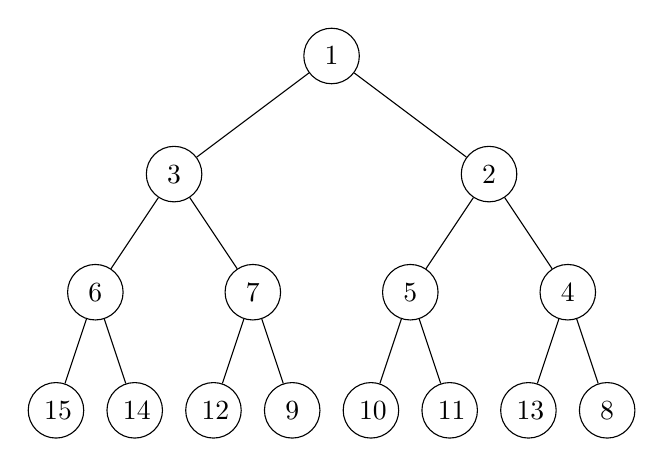
\begin{tikzpicture}[every node/.style={circle, draw=black, text width=0.3cm, align=center},
				   level 1/.style={sibling distance=40mm},
				   level 2/.style={sibling distance=20mm},
				   level 3/.style={sibling distance=10mm}]
\node{1}
	child {node {3}
		child {node {6}
			child {node {15}}
			child {node {14}}
		}
		child {node {7}
			child {node {12}}
			child {node {9}}
		}
	}
	child {node {2}
		child {node {5}
			child {node {10}}
			child {node {11}}
		}
		child {node {4}
			child {node {13}}
			child {node {8}}
		}
	}
;
\end{tikzpicture}
}
\end{center}

Begynner med å slette rot noden 1. Og flytter siste element (8) opp til rot posisjon.

\begin{center}
\scalebox{0.8}{
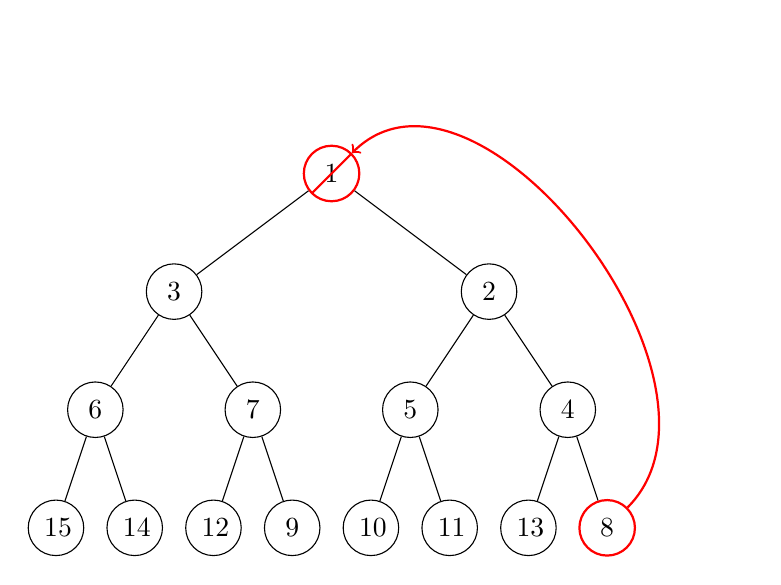
\begin{tikzpicture}[every node/.style={circle, draw=black, text width=0.3cm, align=center},
				   level 1/.style={sibling distance=40mm},
				   level 2/.style={sibling distance=20mm},
				   level 3/.style={sibling distance=10mm}]
\node[draw=red, thick, forbidden sign] (B) {1}
	child {node {3}
		child {node {6}
			child {node {15}}
			child {node {14}}
		}
		child {node {7}
			child {node {12}}
			child {node {9}}
		}
	}
	child {node {2}
		child {node {5}
			child {node {10}}
			child {node {11}}
		}
		child {node {4}
			child {node {13}}
			child {node[draw=red, thick] (A) {8}}
		}
	}
;

\draw[->, red, thick] (A) to [out=45,in=45] (B);
\end{tikzpicture}
}
\end{center}

Får da dette resultatet. Og vi må nå flytte 8 ned til riktig posisjon.

\begin{minipage}{0.5\textwidth}
\scalebox{0.8}{
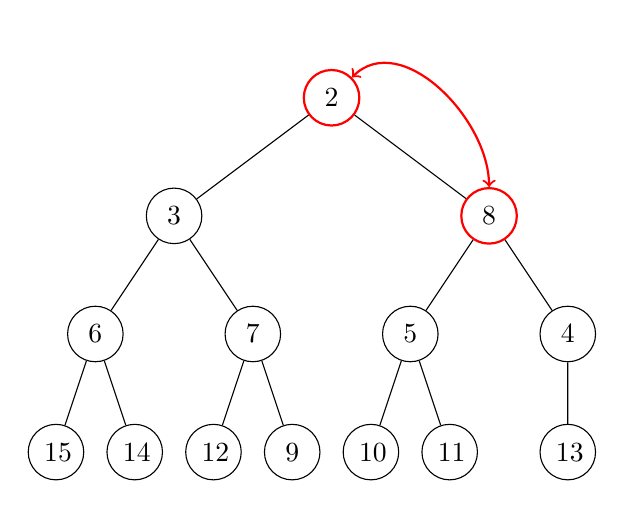
\begin{tikzpicture}[every node/.style={circle, draw=black, text width=0.3cm, align=center},
				   level 1/.style={sibling distance=40mm},
				   level 2/.style={sibling distance=20mm},
				   level 3/.style={sibling distance=10mm}]
\node[draw=red, thick](B){2}
	child {node {3}
		child {node {6}
			child {node {15}}
			child {node {14}}
		}
		child {node {7}
			child {node {12}}
			child {node {9}}
		}
	}
	child {node[draw=red, thick] (A) {8}
		child {node {5}
			child {node {10}}
			child {node {11}}
		}
		child {node {4}
			child {node {13}}
		}
	}
;
\draw[<->, red, thick] (A) to [out=90,in=45] (B);
\end{tikzpicture}
}
\end{minipage}
\begin{minipage}{0.5\textwidth}
\scalebox{0.8}{
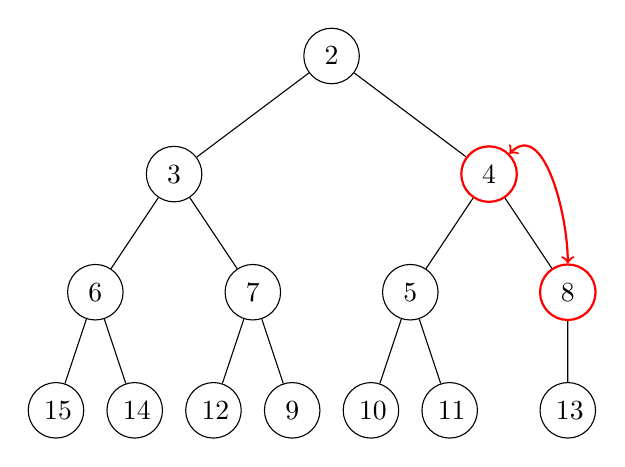
\begin{tikzpicture}[every node/.style={circle, draw=black, text width=0.3cm, align=center},
				   level 1/.style={sibling distance=40mm},
				   level 2/.style={sibling distance=20mm},
				   level 3/.style={sibling distance=10mm}]
\node{2}
	child {node {3}
		child {node {6}
			child {node {15}}
			child {node {14}}
		}
		child {node {7}
			child {node {12}}
			child {node {9}}
		}
	}
	child {node[draw=red, thick] (B) {4}
		child {node {5}
			child {node {10}}
			child {node {11}}
		}
		child {node[draw=red, thick] (A) {8}
			child {node {13}}
		}
	}
;
\draw[<->, red, thick] (A) to [out=90,in=45] (B);
\end{tikzpicture}
}
\end{minipage}


%%% GRAFER %%%
\section{Grafer}

\begin{definition}
\emph{\textbf{Graf}}
En \textbf{graf} $\mathcal{G}$ består av en ikke-tom mengde noder $\mathcal{V}$ og en mengde kanter $\mathcal{E}$, slik at enhvet kant forbinder nøyaktig to noder med hverandre eller en node med seg selv.
\end{definition}

\subsection{Terminologi}
\begin{definition}
\emph{\textbf{Vektet}} En graf er vektet dersom hver kant har en tredje komponent. En verdi langs kanten.
\end{definition}
\begin{definition}
\emph{\textbf{Sti}} En sti gjennom grafen er en sekvens av noder $v_1, v_2, v_3, \dots, v_n$, slik at $(v_i,v_{i+1}) \in \mathcal{E}$ for $1 \leq i \leq n-1$.
\end{definition}
\begin{definition}
\emph{\textbf{Lengde}} Lengden til stien er lik antall kanter på stien.
\end{definition}
\begin{definition}
\emph{\textbf{Løkke}}  Ei løkke i en rettet graf er en vei med lengde $\geq 1$, slik at $v_1=v_n$. Løkken er \textit{enkel} dersom stien er enkel.
\end{definition}
\begin{definition}
\emph{\textbf{Asyklisk}}  En rettet graf er asyklisk dersom den ikke har noen løkker. DAG (Directed, Asyclic Graph).
\end{definition}
\begin{definition}
\emph{\textbf{Sammenhengende}} En urettet graf er sammenhengende dersom det fins en sti fra hver node til alle andre noder.
\end{definition}

\subsection{Topologisk sortering}
\begin{definition}
\emph{\textbf{Topologisk sortering}} En topologisk sortering (topologisk orden) av en rettet graf er en lineær ordning av nodene, slik at for hver rettet kant $\langle u,v \rangle$ fra node $u$ til node $v$, så kommer $u$ før $v$ i ordningen.
\end{definition}
\begin{figure}[h!]
\centering
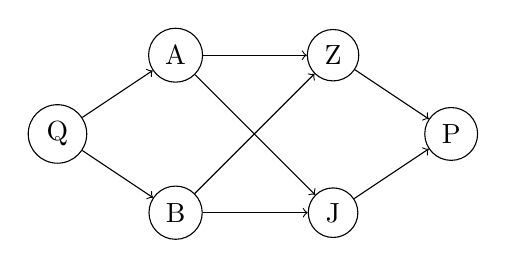
\begin{tikzpicture}[->]
\tikzstyle{vertex} = [circle, draw=black]
\tikzstyle{edge} = [draw=black]

\node[vertex] (A) at (1,0) {A};
\node[vertex] (Q) at (-0.5,-1) {Q};
\node[vertex] (B) at (1,-2) {B};
\node[vertex] (Z) at (3,0) {Z};
\node[vertex] (J) at (3,-2) {J};
\node[vertex] (P) at (4.5,-1) {P};

\draw[edge] (Q) -- (A);
\draw[edge] (Q) -- (B);
\draw[edge] (A) -- (Z);
\draw[edge] (A) -- (J);
\draw[edge] (B) -- (J);
\draw[edge] (B) -- (Z);
\draw[edge] (J) -- (P);
\draw[edge] (Z) -- (P);
\end{tikzpicture}
\caption{Eksempelfigur for topologisk sortering.}
\label{fig:graph}
\end{figure}

I figur \ref{fig:graph} har vi følgende lovlige topologiske sorteringer:

\begin{itemize}
\item
Q, A, B, J, Z, P
\item
Q, B, A, J, Z, P
\item
Q, A, B, Z, J, P
\item
Q, B, A, Z, J, P
\end{itemize}

\subsubsection{Algoritmer} De vanligste algoritmene for topologisk sortering har lineær kjøretid i antall noder, pluss antall kanter; O$(|\mathcal{V}|+|\mathcal{E}|)$. En av disse kommer det et eksempel på her.

\begin{Verbatim}[frame=single]
L <- empty list that will contain the sorted elements
S <- set of all nodes with no incoming edges

while S in non-empty do:
    remove a node n from S
    insert n into L
    for each node m with an edge e from n to m do:
        remove edge e from the graph
        if m had no other incoming edges then:
            insert m into S
if graph has edges then:
    return error (graph has at least one cycle)
else
    return L (a topofically sorted order)
\end{Verbatim}

\subsection{Dijkstra}
\begin{enumerate}
\item
For alle noder, sett avstanden fra startnoden $s$ lik $\infty$. Merk noden som \textit{ukjent}.
\item
Sett avstanden fra $s$ til seg selv lik 0.
\item
Velg en ukjent node $v$ med minimal avstand fra $s$ og marker $v$ som kjent.
\item
For hver ukjente nabonode $w$ til $v$: Dersom avstanden vi får ved å følge veien gjennom $v$, er kortere enn den gamle avstanden til $s$. Redusér avstanden til $s$ for $w$ og sett bakoverpekeren i $w$ til $v$.
\item
Akkurat som for uvektede grafer, ser vi bare etter potensielle forbedringer for naboer som ennå ikke er kjent.
\end{enumerate}

\begin{figure}[h!]
\centering
\scalebox{0.8}{
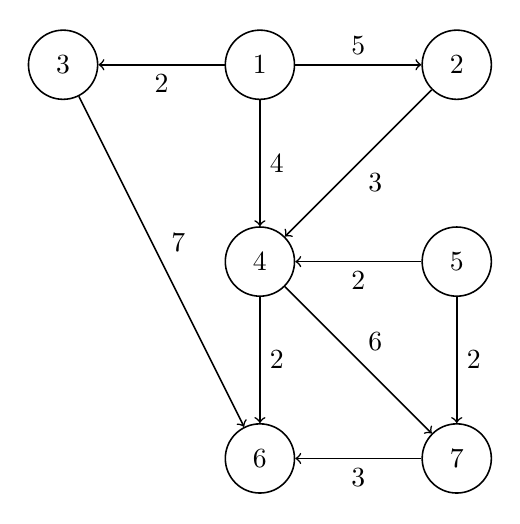
\begin{tikzpicture}[->,auto,node distance=2.5cm,line width=0.2mm]
\node[state] (A) {3};
\node[state] (B) [right of=A] {1};
\node[state] (C) [right of=B] {2};
\node[state] (D) [below of=B] {4};
\node[state] (E) [right of=D] {5};
\node[state] (F) [below of=D] {6};
\node[state] (G) [right of=F] {7}; 

\path 	(A) edge node {7} (F)
		(B) edge node {2} (A)
			edge node {4} (D)
			edge node {5} (C)
		(C) edge node {3} (D)
		(D) edge node {2} (F)
			edge node {6} (G)
		(E) edge node {2} (D)
			edge node {2} (G)
		(G) edge node {3} (F)
;
\end{tikzpicture}
}
\caption{Eksempelgraf for Dijkstra.}
\label{fig:graph2}
\end{figure}

\begin{table}
\centering
\begin{tabular}{c|ccc|ccc|ccc}
&&\textbf{Init}&&&\textbf{1}&&&\textbf{3}\\
V & known & dist. & from&known&dist.&from&known&dist.&from\\
\hline
1 & F & 0 & 0&T&0&0&T&0&0\\
2 & F & -- & 0&F&5&1&F&5&1\\
3 & F & -- & 0&F&2&1&T&2&1\\
4 & F & -- & 0&F&4&1&F&4&1\\
5 & F & -- & 0&F&--&0&F&--&0\\
6 & F & -- & 0&F&--&0&F&9&3\\
7 & F & -- & 0&F&--&0&F&--&0\\
\hline
\hline
&&\textbf{6}&&&\textbf{4}&&&\textbf{7}\\
V & known & dist. & from&known&dist.&from&known&dist.&from\\
\hline
1&T&0&0&T&0&0&T&0&0\\
2&F&5&1&F&5&1&F&5&1\\
3&T&2&1&T&2&1&T&2&1\\
4&F&4&1&T&4&1&T&4&1\\
5&F&--&0&F&--&0&F&--&0\\
6&T&9&3&T&6&4&T&6&4\\
7&F&--&0&F&10&4&T&10&4\\
\hline
\hline
&&\textbf{2}&\\
V & known & dist. & from\\
\cline{1-4}
1&T&0&0\\
2&T&5&1\\
3&T&2&1\\
4&T&4&1\\
5&F&--&0\\
6&T&6&4\\
7&T&10&4\\
\end{tabular}
\label{tab:dijkstra}
\caption{Tabell til Dikjstra-algoritmen på grafen i figur \ref{fig:graph2}.}
\end{table}

\newpage
\paragraph{Algoritmen} Her er pseudokoden for Dijkstra.

\begin{Verbatim}[frame=single]
function Dijkstra (Graph, source):
    for each vertex v in Graph:
        distance[v] := infinity
        visited[v] := false;
        previous[v] := undefined;
    
    distance[source] = 0;
    insert source into Q;

    while Q is not empty:
        u := vertex in Q with smallest distance in distance[] 
                    and has not been visited;
        remove u from Q;
        visited[u] := true;

        for each neighbour v of u:
            alt := distance[u] + dist_between(u,v);
            if alt < dist[v];
                dist[v] := alt;
                previous[v] := u;
                if !visited[v]:
                    insert v into Q;
    return distance;
end function;
\end{Verbatim}

\newpage

\subsection{Prim}
\begin{figure}[h!]
\centering
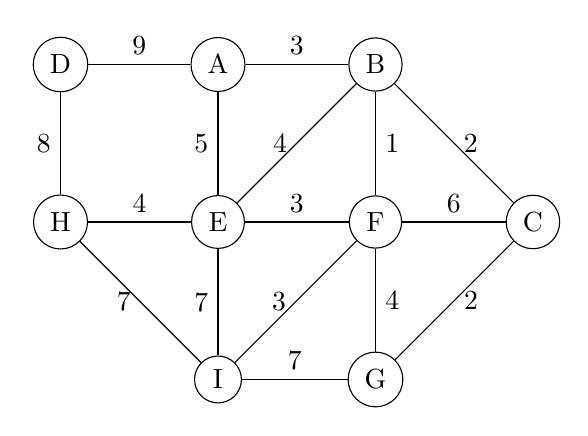
\begin{tikzpicture}
\tikzstyle{vertex} = [circle, draw=black]
\tikzstyle{edge} = [draw=black]
\tikzstyle{selected edge} = [-, red!100]

\node[vertex] (A) at (0,0) {A};
\node[vertex] (B) at (2,0) {B};
\node[vertex] (D) at (-2,0) {D};
\node[vertex] (C) at (4,-2) {C};
\node[vertex] (H) at (-2,-2) {H};
\node[vertex] (E) at (0,-2) {E};
\node[vertex] (F) at (2,-2) {F};
\node[vertex] (I) at (0,-4) {I};
\node[vertex] (G) at (2,-4) {G};

\path (A) edge node [above] {3} (B);
\path (A) edge node [left] {5} (E);
\path (A) edge node [above] {9} (D);
\path (B) edge node [right] {2} (C);
\path (B) edge node [right] {1} (F);
\path (B) edge node [left] {4} (E);
\path (C) edge node [above] {6} (F);
\path (C) edge node [right] {2} (G);
\path (D) edge node [left] {8} (H);
\path (E) edge node [above] {3} (F);
\path (E) edge node [left] {7} (I);
\path (F) edge node [right] {4} (G);
\path (F) edge node [left] {3} (I);
\path (G) edge node [above] {7} (I);
\path (H) edge node [left] {7} (I);
\path (H) edge node [above] {4} (E);
\end{tikzpicture}
\caption{Eksempelgraf for Prim og Kruskal.}
\label{fig:graph3}
\end{figure}

\subsubsection{Framgangsmåte}
\begin{enumerate}
\item
Initialiser et tre med en enkelt node, valgt tilfeldig fra grafen.
\item
Gro treet med én kant (av de kantene som går til en node som ikke er med i treet), finn den kanten med minst vekt og legg den inn i treet.
\item
Gjenta steg 2 til alle nodene er i treet.
\end{enumerate}

\begin{Verbatim}[frame=single]
PRIM(G, w, r) 
  for each u in G.V
    u.key = infinite
    u.parent = NIL
  r.key = 0
  Q = G.V
  while Q is not empty
    u = extract-min(Q)
    for each v in G.Adj[u]
      if (v in Q) and w(u,v) < v.key
        v.parent = u
        v.key = w(u,v)
\end{Verbatim}

Når man utfører Prims algoritme på grafen i figur \ref{fig:graph3}, så blir resultatet følgende:
\begin{figure}[h!]
\centering
\scalebox{0.8}{
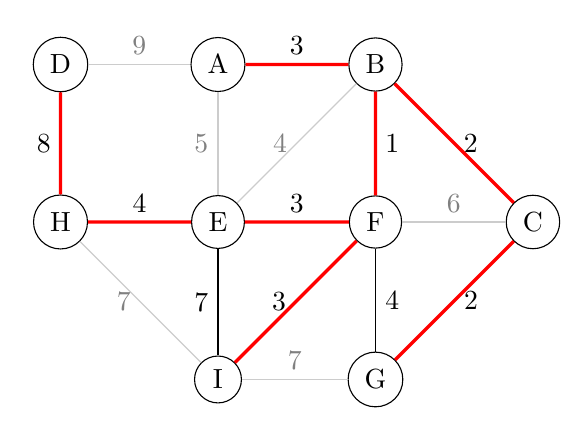
\begin{tikzpicture}
\tikzstyle{vertex} = [circle, draw=black]
\tikzstyle{edge} = [draw=black]
\tikzstyle{selected edge} = [-, red!100, very thick]

\node[vertex] (A) at (0,0) {A};
\node[vertex] (B) at (2,0) {B};
\node[vertex] (D) at (-2,0) {D};
\node[vertex] (C) at (4,-2) {C};
\node[vertex] (H) at (-2,-2) {H};
\node[vertex] (E) at (0,-2) {E};
\node[vertex] (F) at (2,-2) {F};
\node[vertex] (I) at (0,-4) {I};
\node[vertex] (G) at (2,-4) {G};

\path (A) edge node [above] {3} (B);
\path (A) edge[black!20] node [left, gray] {5} (E);
\path (A) edge[black!20] node [above, gray] {9} (D);
\path (B) edge node [right] {2} (C);
\path (B) edge node [right] {1} (F);
\path (B) edge[black!20] node [left, gray] {4} (E);
\path (C) edge[black!20] node [above, gray] {6} (F);
\path (C) edge node [right] {2} (G);
\path (D) edge node [left] {8} (H);
\path (E) edge node [above] {3} (F);
\path (E) edge node [left] {7} (I);
\path (F) edge node [right] {4} (G);
\path (F) edge node [left] {3} (I);
\path (G) edge[black!20] node [above, gray] {7} (I);
\path (H) edge[black!20] node [left, gray] {7} (I);
\path (H) edge node [above] {4} (E);

\draw[selected edge] (D) -- (H) -- (E) -- (F) -- (I) -- (F) -- (B) -- (A) -- (B) -- (C) -- (G);
\end{tikzpicture}
}
\caption{Eksempelgraf \ref{fig:graph3} etter Prims algoritme.}
\label{fig:prim}
\end{figure}

\begin{table}
\centering
\begin{tabular}{ccc}
&avs.&fra\\
A&0&--\\
B&3&A\\
C&2&B\\
D&8&H\\
E&3&F\\
F&1&B\\
G&2&C\\
H&4&E\\
I&3&F\\
\cline{2-2}
&26&\\
\cline{2-2}
\end{tabular}
\caption{Tabell for Prims algoritme på figur \ref{fig:prim}.}
\end{table}

\textbf{MERK:} løsningen i figur \ref{fig:prim} er \textit{ikke} unik. Eneste måten man kan få et unikt resultat er om alle vektene på kantene er unike. Det samme gjelder for Kruskal.

\subsection{Kruskal}
\subsubsection{Framgangsmåte}
\begin{itemize}
\item
Lag en \textit{skog} $\mathcal{F}$ (en sett med trær), hver hver node i grafen er et separat tre.
\item
Lag et sett $\mathcal{S}$ som inneholder alle kantene til grafen.
\item
Så lenge $\mathcal{S}$ ikke er tom og $\mathcal{F}$ ikke ennå er et spanning-tre:
\begin{itemize}
\item
Fjern en kant men lavest vekt fra $\mathcal{S}$.
\item
Hvis kanten kobler to forskjellige trær, legg den i skogen slik at de to blir ett tre.
\end{itemize}
\end{itemize}
Når algoritmen er ferdig, så former skogen et minimum spanning-tre for grafen. 

\begin{Verbatim}[frame=single]
KRUSKAL (G):
  A = empty
  for each v in G.V:
    MAKE-SET(v)
  for each (u,v) ordered by weight(u,v), increasing:
    if FIND-SET(u) not in FIND-SET(v):
      A = A union {(u,v)}
      UNION(u,v)
  return A
\end{Verbatim}

\begin{figure}[h!]
\centering
\scalebox{0.8}{
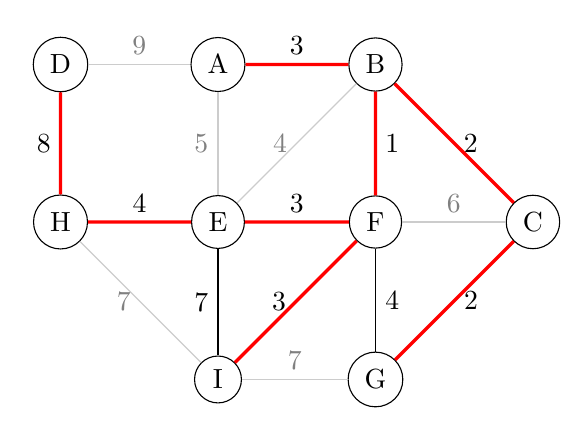
\begin{tikzpicture}
\tikzstyle{vertex} = [circle, draw=black]
\tikzstyle{edge} = [draw=black]
\tikzstyle{selected edge} = [-, red!100, very thick]

\node[vertex] (A) at (0,0) {A};
\node[vertex] (B) at (2,0) {B};
\node[vertex] (D) at (-2,0) {D};
\node[vertex] (C) at (4,-2) {C};
\node[vertex] (H) at (-2,-2) {H};
\node[vertex] (E) at (0,-2) {E};
\node[vertex] (F) at (2,-2) {F};
\node[vertex] (I) at (0,-4) {I};
\node[vertex] (G) at (2,-4) {G};

\path (A) edge node [above] {3} (B);
\path (A) edge[black!20] node [left, gray] {5} (E);
\path (A) edge[black!20] node [above, gray] {9} (D);
\path (B) edge node [right] {2} (C);
\path (B) edge node [right] {1} (F);
\path (B) edge[black!20] node [left, gray] {4} (E);
\path (C) edge[black!20] node [above, gray] {6} (F);
\path (C) edge node [right] {2} (G);
\path (D) edge node [left] {8} (H);
\path (E) edge node [above] {3} (F);
\path (E) edge node [left] {7} (I);
\path (F) edge node [right] {4} (G);
\path (F) edge node [left] {3} (I);
\path (G) edge[black!20] node [above, gray] {7} (I);
\path (H) edge[black!20] node [left, gray] {7} (I);
\path (H) edge node [above] {4} (E);

\draw[selected edge] (D) -- (H) -- (E) -- (F) -- (I) -- (F) -- (B) -- (A) -- (B) -- (C) -- (G);
\end{tikzpicture}
}
\caption{Eksempelgraf \ref{fig:graph3} etter Kruskals algoritme.}
\label{fig:kruskal}
\end{figure}

\begin{tabular}{r|ccccccccl}
\textbf{Kant} & FB&BC&CG&FI&FE&BA&EH&HD\\
\cline{1-9}
\textbf{Vekt}&1&2&2&3&3&3&4&8&$\Rightarrow$26
\end{tabular}

% Dybde-først
\subsection{Dybde-først}
Dette er klassisk graf-traversering, generalisering av prefiks traversering for trær. Gitt start node $v$: rekursivt traverser alle nabonodene.
\begin{lstlisting}
public void depthFirstSearch(Node v)
	v.marked = true;
	for <each neighbour w to v>
		if (!w.marked)
			depthFirstSearch(w);
\end{lstlisting}

\subsection{Biconnectivity}
\theoremstyle{mytheoremstyle}
\newtheorem{biconnect}{Definisjon}[subsection]
\begin{biconnect}
En sammenhengende urettet graf er \textbf{bi-connected} hvis det ikke er noen noder som ved fjerning gjør at grafen blir usammenhengende. Slike noder heter cut-vertices eller articulation points.
\end{biconnect}

\begin{figure}[h!]
\centering
\scalebox{0.7}{
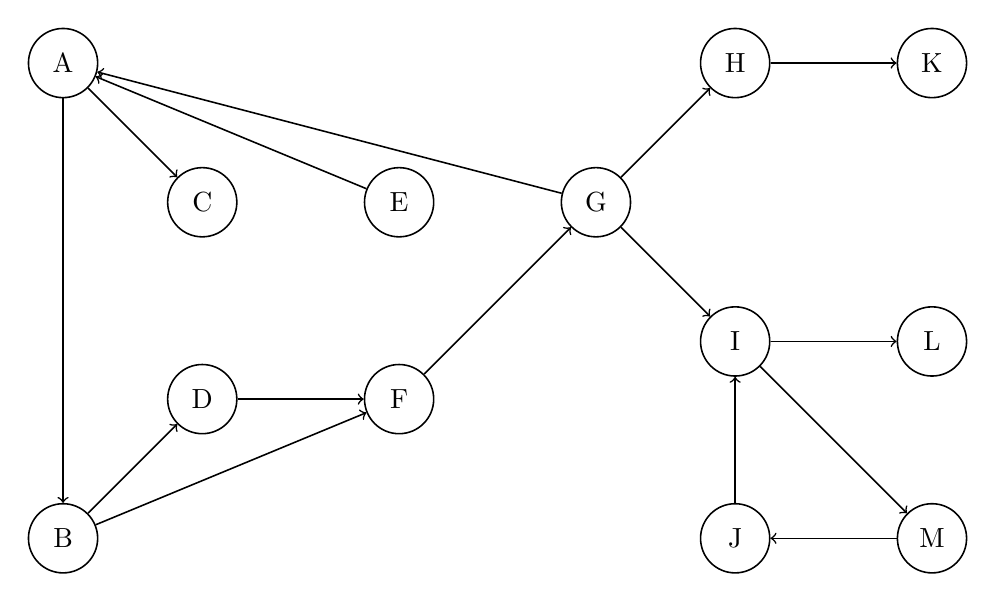
\begin{tikzpicture}[->,auto,node distance=2.5cm,line width=0.2mm]
\node[state] (A) {A};
\node[state] (C) [below right of=A] {C};
\node[state] (E) [right of=C] {E};
\node[state] (G) [right of=E] {G};
\node[state] (H) [above right of=G] {H};
\node[state] (K) [right of=H] {K};
\node[state] (D) [below of=C] {D};
\node[state] (F) [right of=D] {F};
\node[state] (I) [below right of=G] {I};
\node[state] (L) [right of=I] {L};
\node[state] (B) [below left of=D] {B};
\node[state] (J) [below of=I] {J};
\node[state] (M) [right of=J] {M};

\path 	(A) edge node {} (B)
			edge node {} (C)
		(B) edge node {} (D)
			edge node {} (F)
		(D) edge node {} (F)
		(E) edge node {} (A)
		(F) edge node {} (G)
		(G) edge node {} (I)
			edge node {} (H)
			edge node {} (A)
		(H) edge node {} (K)
		(I) edge node {} (L)
			edge node {} (M)
		(J) edge node {} (I)
		(M) edge node {} (J)
;
\end{tikzpicture}
}
\caption{Eksempelgraf for bi-connectivity.}
\label{fig:graphbi}
\end{figure}

Grafen i figur \ref{fig:graphbi} er \textit{ikke} bi-connected, fordi nodene A, I, G og H er articulation points.

\subsubsection{DFS spanning-tre av figur \ref{fig:graphbi}}
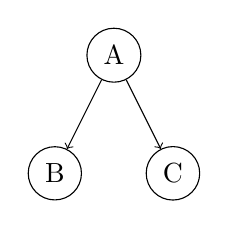
\begin{tikzpicture}[->, every node/.style={draw=black, circle}]
\node{A}
	child {node {B}}
	child {node {C}};
\end{tikzpicture}


\subsection{Strongly connected components (SCC)}
\theoremstyle{mytheoremstyle}
\newtheorem{scc}{Definisjon}[subsection]
\begin{scc}
Gitt en rettet graf $\mathcal{G} = (\mathcal{V}, \mathcal{E})$. En \textbf{strongly connected component} av $\mathcal{G}$ er et maksimalt sett av noder $U \subseteq \mathcal{V}$. For alle $u_1, u_2 \in U$ har vi at $u \rightarrow^*u_2$ og $u_2\rightarrow^*u_1$.
\end{scc}


\section{Kombinatorisk søk}
\section{Rekursjon}

%%% TEKSTALGORITMER %%%
\section{Tekstalgoritmer}

% Brute force
\subsection{Brute force}
Brute force metoden sjekker en og en karakter i teksten med nålen, og flytter med 1 om det er mismatch.

\subsubsection{Analyse}
Worst case så får vi mismatch $(n-m)$ ganger og suksess $(n-m)+1$ ganger. Totale sammenligninger er $((n-m)+1 \times m)$ som gir kjøretid O($n^2$).

% Boyer Moore
\subsection{Boyer Moore}
\begin{itemize}
\item
Først må man lage «bad match table».
\item
Sammenligne nålen med teksten, starter med karakteren lengst til høyre i nålen.
\item
Hvis mismatch, flytt nålen fram iht. verdien i tabellen.
\end{itemize}

\subsubsection{Eksempel}
\begin{description}
\item[Pattern (nål)] tooth
\item[Tekst] trusthardtoothbrushes
\end{description}

\paragraph{1.} Konstruere «bad match table». 
\begin{center}
\texttt{value = length - index - 1}
\end{center}
Alle andre bokstaver har verdi lik lengden.
\begin{center}
\begin{tabular}{rccccc}
&T&O&O&T&H\\
index:&0&1&2&3&4\\
\end{tabular}
\end{center}
Lengden på denne nålen er 5. Finner verdiene ved å bruke \texttt{value = length - index - 1}.
\begin{center}
\begin{tabular}{cccl}
T = & $5-0-1$&= 4\\
O = & $5-1-1$&= 3\\
O = & $5-1-2$&= 2&Erstatter her forrige verdi av O med ny verdi til O.\\
T = &$5-3-1$& = 1&Erstatter her forrige verdi av T med ny verdi til T.\\
H = &5 &&Verdien skal ikke være mindre enn 1. Får da verdi lik lengden.\\
\end{tabular}

\begin{tabular}{l|llll}
Bokstav&T&O&H&$*$\\
\hline
Verdi&1&2&5&5\\
\end{tabular}
\end{center}

\scalebox{0.9}{
\begin{tabular}{cccccccccccccccccccccc}
&T&R&U&S&\textcolor{red}{T}&\textcolor{red}{H}&A&R&D&T&\textcolor{red}{O}&O&\textcolor{red}{T}&H&B&R&U&S&H&E&S\\
\textbf{1.}&T&O&O&T&\textcolor{red}{H}\\
\textbf{2.}&&T&O&\textcolor{red}{O}&\textcolor{dkgreen}{T}&\textcolor{dkgreen}{H}\\
\textbf{3.}&&&&&&&T&O&O&T&\textcolor{red}{H}\\
\textbf{4.}&&&&&&&&&T&O&O&T&\textcolor{red}{H}\\
\textbf{5.}&&&&&&&&&&\textcolor{dkgreen}{T}&\textcolor{dkgreen}{O}&\textcolor{dkgreen}{O}&\textcolor{dkgreen}{T}&\textcolor{dkgreen}{H}\\
\end{tabular}
}

I steg \textbf{1.} får vi mismatch på H, fordi den ikke er det samme som T. Da må vi slå opp i tabellen på den bokstaven som \textbf{\textit{vi møter i teksten}}, og hoppe fram tilsvarende antall steg. I første tilfellet skal vi hoppe 1 plass fram (for 1 er verdien til T). 

Sjekker på nytt i steg \textbf{2.}, her får vi match på T og H, men mismatch på O. Da hopper vi S-plasser frem. Siden S ikke er med i tabellen vår (eller den er med som $*$, som er alle andre bokstaver), så hopper vi 5 plasser frem.

I steg \textbf{3.} får vi mismatch på H mot O, og må hoppe O-plasser frem---altså 2. I steg \textbf{4.} er det mismatch mellom H og T, vi hopper T-plasser frem---altså 1. Og vips! Så har vi funnet nålen i teksten vår!

\subsubsection{Analyse}
Worst case er det samme som brute force. Input tekst $1^n$ kjører $n$ ganger, og nål $011\dots1$ kjører $m$ ganger. Dette gir O($nm$). Best case har input tekst $1^n$ og nål $0^m$, som gir O($n/m$). Average case er O($m/|\Sigma|$), raskere enn brute force.





\newpage

\begin{thebibliography}{}

\bibitem{redblack}
  Unknown,
  \emph{RedBlackBST.java}.
  algs4.cs.princeton.edu,
  \url{http://algs4.cs.princeton.edu/33balanced/RedBlackBST.java.html}

\bibitem{bm}
  Unknown,
  \emph{Boyer Moore Horspool Algorithm}.
  \url{https://www.youtube.com/watch?v=PHXAOKQk2dw}



\end{thebibliography}



\newpage

\listoftables
\listoffigures

\end {document}